\chapter{\IfLanguageName{dutch}{Stand van zaken}{State of the art}}%
\label{ch:stand-van-zaken}

In dit hoofdstuk van de bachelorproef zullen we dieper ingaan op het concept van een microservices-architectuur. Dit zal gebeuren aan de hand van een relevante literatuurstudie. Allereerst zal uitgelegd worden wat een monolithische architectuur is en wat typerend is aan deze stijl van software ontwikkeling. Vervolgens wordt uitgelegd wat een microservices-architectuur is en hoe deze architectuur verschilt van de klassieke, monolithische aanpak. Daarna worden Docker en Kubernetes van naderbij bekeken, twee essentiële tools voor het uitwerken van de PoC. Tot slot worden enkele relevante termen uitgebreider behandeld die de werking en structuur van microservices definiëren. Op basis van de informatie uit dit hoofdstuk zal duidelijk worden wat er allemaal komt kijken tijdens het ontwerpen van een proof-of-concept (PoC) in een later deel van de bachelorproef.

\section{Wat is een monolithische architectuur?}

De monolithische architectuur is door de jaren heen een succesvolle keuze geweest voor softwareontwikkelaars \autocite{Gos2020}. Bij deze aanpak van software ontwikkeling bestaat een applicatie uit verscheidene componenten. Voorbeelden van componenten zijn authenticatie en authorizatie, productbeheer, klantenbeheer enz. Deze componenten bevinden zich in een monolithische architectuur dan in één en hetzelfde programma.

\begin{figure}[H]
  \centering
  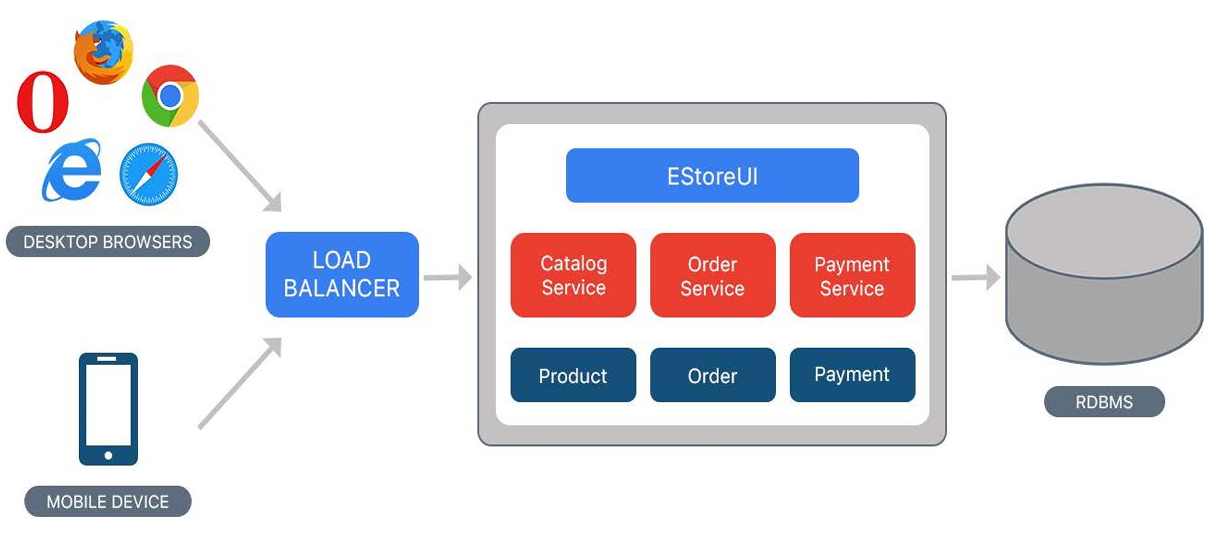
\includegraphics[width=0.85\textwidth]{MonolithischeArchitectuur.png}
  \caption[Voorstelling van een monolitische architectuur]{\label{fig:monolithische architectuur}Voorbeeld van een monolithische architectuur. Deze afbeelding toont de architectuur van een applicatie die de bedrijfslogica voor een e-commerce demonstreert \autocite{Gos2020}.}
\end{figure}

De bovenstaande afbeelding (Figuur \ref{fig:monolithische architectuur}) verduidelijkt de interne structuur van een monolithische applicatie. In deze representatie zien we een EStoreUI component die fungeert als de grafische interface waarmee gebruikers kunnen interageren met de applicatie. Daaronder zijn 3 services gedefiniëerd, namelijk de Catalog Service, Order Service en Payment Service. Elk van deze 3 services is verantwoordelijk voor het respectievelijke bedrijfsproces. Tot slot zijn alle services verbonden met eenzelfde relationele database (RDBMS). Deze verschillende componenten bevinden zich in een monolithische architectuur dan ook binnen dezelfde applicatie.\newline

Een kenmerkend aspect van een monolithische applicatie is de gelaagde structuur, waarbij de grafische interface bovenop verschillende services is opgebouwd en waar er slechts 1 databank is die gedeeld wordt door alle services \autocite{Velepucha2023}. Deze architectuur staat ook beter bekend als het 3-lagenmodel, waarbij de opbouw van een applicatie wordt opgedeeld in diverse lagen. De volgende lagen kunnen geïdentificeerd worden:

\begin{itemize}
	\item \textbf{Presentatielaag}: binnen deze laag vinden we de code die het mogelijk maakt voor gebruikers om met de applicatie te interageren.
	\item \textbf{Business laag}: deze laag is specifiek ontworpen met het oog op het implementeren van bedrijfsfunctionaliteit en validatie.
	\item \textbf{Datalaag}: hierin worden alle interacties met de data-opslag gedefinieerd alsook de interacties met externe services die nodig zijn voor de applicatie.
\end{itemize}

De monolithische architectuur brengt een aantal voordelen met zich mee, zoals eenvoudige implementatie en gemakkelijke testbaarheid \autocite{Li2022}. Toch zijn er ook een aantal mindere aspecten aan deze software architectuur, voornamelijk wanneer de applicatie dient te groeien. Naarmate bedrijven groeien en hun software uitbreiden, kan de toenemende grote van de codebase leiden tot verschillende problemen, zoals schaalbaarheid en onderhoudbaarheid \autocite{Wei2025}. Wijzigingen in de functionaliteiten of bugfixes kunnen bijvoorbeeld onverwachte gevolgen hebben voor de gehele applicatie. Daarnaast heeft de sterke opkomst van cloud computing de voordelen van een monolithische architectuur opmerkelijk verminderd. Cloud-gebaseerde oplossingen vereisen vaak schaalbaarheid en flexibiliteit. Deze 2 factoren sluiten minder goed aan bij de klassieke, monolithische applicatie. Volgens \textcite{Wei2025} heeft deze evolutie dan ook geleid tot een toenemende interesse in microservices.

\section{Wat is een microservices-architectuur?}

Succesvolle softwaresystemen groeien in de loop van de tijd vaak in omvang en complexiteit \autocite{Abgaz2023}. Dit door de toevoeging van verschillende functionaliteiten, wat kan resulteren in sterk gekoppelde, maar toch minder samenhangende componenten. Als gevolg hiervan hebben monolithische applicaties vaak beperkingen op het gebied van schaalbaarheid, onderhoud en prestaties. In de huidige bedrijfsomgevingen is de nood om schaalbare applicaties te ontwikkelen essentieel, wegens de opkomst van nieuwe technologieën en de vraag om zowel menselijke als technologische middelen te optimaliseren \autocite{Nayim2023}.\newline

Een van de allereersten die een definitie voor microservices gaven waren \textcite{Lewis2014}. Zij beschreven in hun blogpost de microservices-architectuur als een software architectuur waarbij één enkele applicatie bestaat uit verschillende, kleinere services. Deze kleinere services kunnen onafhankelijk van elkaar werken en communiceren met elkaar door gebruik te maken van bijvoorbeeld Hypertext Transfer Protocol (HTTP) of een Application Programming Interface (API). Wanneer we dan kijken naar een recentere beschrijving van dit concept, dan benadrukken \textcite{Velepucha2023} dat de microservices-architectuur een vorm is van een \hyperref[sec:distributed systems]{gedistribueerd systeem} waarin services onafhankelijk kunnen werken. Daarnaast voegen ze er nog aan toe dat elke service binnen deze architectuur een specifieke bedrijfsfunctionaliteit dient te vervullen.

\begin{figure}[H]
	\centering
	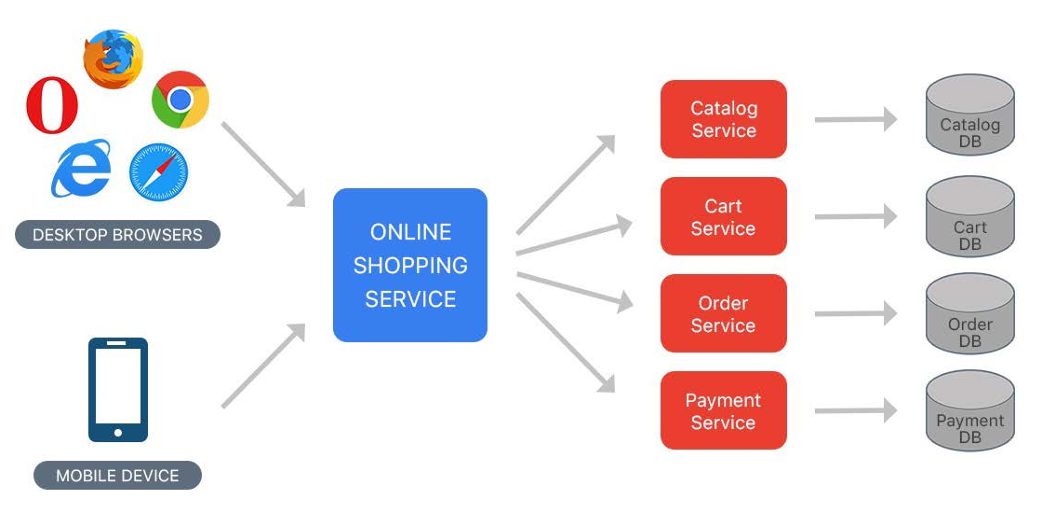
\includegraphics[width=0.75\textwidth]{MicroservicesArchitectuur.png}
	\caption[Voorstelling van een microservices architectuur]{\label{fig:microservices architectuur}Voorbeeld van een microservices architectuur. Deze afbeelding toont een vereenvoudigde representatie van een applicatie met microservices \autocite{Gos2020}.}
\end{figure}

Hierboven wordt de kern van de microservices-architectuur weergegeven. Eerder in dit hoofdstuk zagen we een gelijkaardige representatie, maar dan voor een monolithische architectuur. Daarin benadrukten we dat alle services binnen eenzelfde applicatie behoorden. Hier zien we nu dat alle 4 de services los van elkaar staan en dat ze toegankelijk zijn via één dirigerende service. Een ander opvallend aspect van deze software architectuur, die bij de bovenstaande definities van microservices niet vermeld werd, is dat elke service zijn eigen databank heeft.\newline

De belangrijkste principes waarmee rekening mee moet gehouden worden bij het uitwerken van dit type software architectuur zijn volgens \textcite{Blinowski2022}:

\begin{itemize}
	\item \textbf{Één verantwoordelijkheid per service} - Volgens de SOLID-principes\footnote{Dit is een TEST!} moet elke service ter allen tijde slechts en alleen één verantwoordelijkheid hebben. Nooit mogen twee of meerdere services eenzelfde verantwoordelijkheid delen.
	\item \textbf{Microservices zijn autonoom} - Elke microservice is volledig verantwoordelijk voor het uitvoeren van een specifieke bedrijfsfunctionaliteit. Hierdoor bevatten ze alle benodigde afhankelijkheden, zoals bibliotheken.
	\item \textbf{Services zijn volwaardige componenten} - Eindpunten worden ter beschikking gesteld als API's en verbergen de interne implementatiedetails. De logica, architectuur en gebruikte technologieën blijven volledig verborgen achter de API.
\end{itemize}

Daarnaast vindt \textcite{Blinowski2022} het relevant om te vermelden dat de manier waarop microservices communiceren significant verschilt van de benadering die de \hyperref[sec:SOA_architectuur]{Service Oriented Architecture (SOA)} neemt. Over de relatie tussen microservices en SOA bestaat echter geen eenduidige overeenstemming \autocite{Li2021}. Sommige voorstanders van microservices beschouwen het als een volledig nieuwe architecturale stijl, terwijl aanhangers van SOA microservices eerder zien als een specifieke implementatievorm binnen SOA.

\subsection{Karakteristieken van microservices}

\textcite{Bakshi2017} beschrijft in zijn gepubliceerde artikel verscheidene kenmerken van microservices. Hieronder zijn enkele relevante kenmerken uitgeschreven.

\subsubsection{Services opdelen in componenten}

Microservices maken gebruik van componenten die onafhankelijk vervangbaar en uitbreidbaar zijn. Deze componenten communiceren via mechanismen zoals webservices of remote procedure calls (RPC).

Het grootste voordeel bij het werken met aparte componenten is dat deze onafhankelijk kunnen worden ingezet, waardoor, indien nodig, wijzigingen aan het ene component kunnen worden doorgevoerd zonder de andere te beïnvloeden.

\subsubsection{Georganiseerd rond bedrijfsfunctionaliteiten}

Microservices worden ontworpen met een focus op bedrijfsfunctionaliteiten, zoals ook al eerder werd aangehaald. Hierbij moet gekeken worden naar een brede implementatie van software voor een specifiek bedrijfsdomein. Deze implementatie omvat een gebruikersinterface, persistente opslag en externe samenwerkingen.

Dit resulteert in cross-functionele teams, waarbij skills met betrekking tot gebruikservaring, databanken en projectmanagement essentieel zijn.

\subsubsection{Gebruik van continuous Integration/Continuous Deployment}

Applicatieontwikkeling met microservices maakt gebruik van het CI/CD proces, waarbij software voordurend wordt ontwikkeld en functies worden toegevoegd. Dit proces omvat een ontwikkel-, test-, staging- en productieomgeving.

De monolithische aanpak legt voornamelijk de focus op het afleveren van compleet afgewerkte software. Deze software wordt overgedragen aan de klant en het projectteam gaat over naar het nieuwe project.

\subsubsection{Smart endpoints, dumb pipes}

Traditioneel wordt er voor communicatiesysteem gekeken naar een \hyperref[sec:ESB]{Enterprise Services Bus (ESB)}. Microservices daarentegen gebruiken communicatieprotocollen zoals Representational State Transfer (REST). Hierdoor bevindt de logica zich in de services (smart endpoints) en gebeurt de communicatie op een eenvoudige manier (dumb pipes).

\subsubsection{Fouttolerantie en monitoring}

Een microservices-architectuur moet ontworpen worden zodat wanneer een individuele service uitvalt de applicatie als geheel niet faalt. Real-time monitoring speelt hierin een cruciale rol, maar dit is buiten de scope van deze bachelorproef.

\subsubsection{Decentralisatie van logica en data}

Een belangrijk hulpmiddel bij het maken van services is het Domain Driven Design (DDD) principe. Binnen DDD wordt een complex domein opgesplitst in kleinere contexten, die elk een eigen verantwoordelijkheid hebben. Deze contexten werken samen, maar zijn onafhankelijk van elkaar.

Daarnaast decentraliseert een microservices-architectuur de manier waarop data wordt opgeslagen en beheerd. Monolithische applicaties gebruiken grotendeels één databank. Microservices opteren om elke service zijn eigen databank te laten beheren. Deze aanpak wordt ook wel \hyperref[sec:Polyglot Persistence]{Polyglot Persistence} genoemd.

\subsubsection{Flexibiliteit in technologiekeuze}
\label{sec:flexibiliteit_technologiekeuze}

Doordat services onafhankelijk zijn, kunnen deze ontwikkeld worden met de meest geschikte programmeertaal of technologie, zoals Node.js, Python, Java of C++.

\section{Docker}

Docker is een populaire containertechnologie die applicaties in containers draait zonder hardwarevirtualisatie, hierdoor zijn ze sneller en efficiënter dan virtuele machines \autocite{Kim2022}. Met behulp van Docker kunnen applicaties als Docker-images op elke cloudhost met een Docker-omgeving uitgevoerd worden. Dit maakt het mogelijk om applicaties tussen verschillende cloudproviders eenvoudig te migreren en te gebruiken, wat voorkomt dat je aan één bepaalde vendor vast zit.\newline

Vroeger werd softwareontwikkeling gekenmerkt door een scheiding tussen ontwikkelaars en systeembeheerders \autocite{Schenker2023}. Nadat de ontwikkelaars een applicatie voltooiden werd deze overgedragen aan de systeembeheerders. Zij waren dan verantwoordelijk voor de installatie en werking op de productieservers. Deze manier van werken bracht echter heel wat uitdagingen met zich mee, vooral binnen grotere bedrijven waar meerdere teams applicaties met verschillende structuren ontwikkelden. Vaak leidden verschillen in frameworks, bibliotheken en versies tot problemen in verband met compatibiliteit, waardoor updates en implementaties dikwijls tijdrovend werden.

Om deze uitdagingen te voorkomen, werden allereerst virtuele machines (VMs) gebruikt. Door het gebruik van VMs werd het mogelijk om applicaties geïsoleerd van elkaar te draaien, waardoor de compatibiliteitsproblemen verminderden. Desondanks dit voordeel moest elke VM een volledig besturingssysteem hebben, wat er dan weer voor zorgde dat VMs een zeer zware oplossing waren.

Een lichter alternatief was Docker met de containertechnologie. \textbf{Docker-containers} verpakken een applicatie en zijn dependencies in een licht formaat. Dit zorgt ervoor dat applicaties in elke omgeving kunnen functioneren. Bovendien maakt Docker het mogelijk om sneller en efficiënter software te ontwikkelen, testen en implementeren, waardoor bedrijven flexibeler kunnen releasen.\newline

Een \textbf{Docker-image} kan je vergelijken met een sjabloon dat alle benodigde bestanden en informatie bevat om een container te maken \autocite{Huang2018}. Een image definieert wat er moet zijn om de applicatie te kunnen starten, maar het heeft zelf geen fysieke aanwezigheid op het systeem of toegang tot systeembronnen zoals CPU, geheugen of opslag.

Een Docker-container daarentegen heeft wel een fysieke aanwezigheid op het systeem en heeft een eigen IP-adres en netwerkpoorten. Een container kan gezien worden als een werkende instantie van een image.

\begin{figure}[H]
	\centering
	\includegraphics[width=0.65\textwidth]{Docker\_VM.png}
	\caption[Voorstelling van Docker tegenover een Virtuele Machine]{\label{fig:Docker vs VM}In bovenstaande afbeelding wordt de opstelling van een Docker container tegenover een Virtuele Machine gezet \autocite{Kim2022}.}
\end{figure}

Figuur \ref{fig:Docker vs VM} toont een vereenvoudigde vergelijking van twee methoden voor het opzetten van een applicatie. Aan de linkerkant wordt er gebruik gemaakt van een virtuele machine die draait op een server of computer, en aan de rechterkant worden Docker-containers gebruikt. Het belangrijkste verschil is dat bij virtuele machines een apart besturingssysteem moet worden geïnstalleerd. Dit besturingssysteem moet dan op zijn beurt de applicatie en alle andere onderdelen beheren voor de werking ervan. Voor deze bachelorproef is het voldoende om het verschil tussen Virtuele machine en Docker te kennen. Een diepere kijk op virtualisatie ligt buiten de scope van deze bachelorproef.

\section{Kubernetes}

Kubernetes is een open-source orkestratiesysteem voor het beheren van applicaties in containers \autocite{Turin2023}. Met behulp van Kubernetes kunnen applicaties onderhouden en geschaald worden. Binnen Kubernetes draait alles om pods. Deze pods bevatten op zich dan nog verschillende componenten om services te beheren. 

\begin{itemize}
	\item \textbf{Containers en pods} - Kubernetes gebruikt containers, zoals Docker-containers om pods te draaien. Een pod is het kleinste component binnen Kubernetes en bevat één of meedere containers die dan samen op een node worden geplaatst. Pods communiceren onderling via IP-adressen, maar deze adressen zijn niet statisch en worden telkens toegekend wanneer de pods herstarten.
	\item \textbf{Nodes en clusterbeheer} - Een cluster in Kubernetes bestaat uit nodes. De master node regelt de coördinatie tussen de verschillende nodes. Worker nodes draaien de pods en hebben CPU- en geheugencapaciteiten. Om de pods toe te kennen aan de nodes is er de scheduler, die op basis van beschikbare resources en de vereisten van de applicatie de pods zal verdelen.
	\item \textbf{Services} - Een service is een verzameling van pods die eenzelfde functie uitvoeren en als één entitiet worden gepresenteerd via een service-endpoint. Dit maakt het eenvoudiger om verzoeken naar de juiste back-end containers te routeren, zelfs wanneer deze veranderen of worden vervangen. Standaard zijn services alleen intern toegankelijk, maar ze kunnen ook extern beschikbaar gemaakt worden.
\end{itemize}

Kubernetes zorgt ervoor dat pods automatisch worden aangemaakt en opnieuw gestart \autocite{Vayghan2021}. Pods zijn dynamisch: ze kunnen worden verplaatst of verwijderd, en hun IP-adressen veranderen voortdurend. Dit heeft een negatieve invloed op de communicatie tussen pods. Om dit tegen te gaan, krijgen pods labels die bijgehouden blijven, zelfs wanneer ze opnieuw worden aangemaakt. Daarnaast maakt Kubernetes gebruik van services, die een vast IP-adres hebben en netwerkverkeer verdelen over de verschillende pods, waardoor stabiele en efficiënte communicatie tussen componeneten mogelijk wordt.

\section{Relevante termen}

In dit gedeelte van de literatuurstudie gaan we dieper in op de begrippen die eerder al aan bod zijn gekomen. Hierdoor zal het duidelijk worden wat deze begrippen inhouden en hoe deze relevant zijn voor dit onderzoek.

\subsection{Distributed Systems}
\label{sec:distributed systems}

In de literatuur zijn al diverse definities terug te vinden over gedistribueerde systemen, maar geen enkele stemmen overeen met elkaar \autocite{Steen2018}. Daarom definiëren \textcite{Steen2018} distributed systems als een verzameling van autonome, rekenkundige elementen die voor de gebruikers als één samenhangend systeem lijkt te functioneren.

Volgens hen benadrukt deze definitie twee kenmerken van gedistribueerde systemen. Het eerste kenmerk is dat een gedistribueerd systeem bestaat uit een verzameling van rekenkundige elementen die onafhankelijk van elkaar kunnen functioneren. Deze elementen kunnen zowel hardware-apparaten als softwareprocessen zijn. Het tweede kenmerk is dat gebruikers, zowel mensen als andere applicaties, de indruk hebben dat ze met één samenhangend systeem te maken hebben. Dit benadrukt dat de elementen op de een of andere manier moeten samenwerken. Hoe deze samenwerking tot stand komt is de kern van gedistribueerde systemen aldus \textcite{Steen2018}.

Gedistribueerde systemen zijn de afgelopen twee decennia in trek wegens de groeiende vraag naar onafhankelijke ontwikkeling en implementatie van webapplicaties \autocite{Raj2021}. Dit soort systemen worden essentieel voor het snel leveren van diensten met behulp van continious integration en continuous development (CI/CD). Een van de basisarchitecturen binnen gedistribueerde systemen is Service-Oriented Architecture (SOA), waarbij services centraal staan in het ontwerp.

\subsection{Service-Oriented Architecture}
\label{sec:SOA_architectuur}

Een service-oriented architectuur (SOA) wordt gedefinieerd als een architectuurstijl dat is ontworpen voor het creëren van een losse verbinding tussen systemen \autocite{Rojas2021}. De SOA stijl bestaat uit serviceproviders en -consumenten die met elkaar samenwerken via een vooraf overeengekomen interface. 

Op deze manier vermindert de tijd, inspanningen en kosten die nodig zijn om oplossingen te onderhouden en uit te breiden. De basiscomponenten zijn onafhankelijk verbonden, interoperabel, gedistribueerd en de connectoren zijn synchrone of asynchrone berichtsmechanismen.\newline

Volgens \textcite{Muhardany2020} is SOA een ontwerparchitectuur die helpt bij het bijsturen van de bedrijfsstrategie. SOA helpt voornamelijk bedrijven om hun strategie en diensten op een georganiseerde manier te ontwerpen. Dit betekent dat SOA niet alleen een technische impact heeft, maar ook een strategische.

De basis van SOA bestaat uit drie hoofdcomponenten \autocite{Muhardany2020}:

\begin{itemize}
	\item \textbf{Bedrijfsarchitectuur} - De bedrijfsarchitectuur heeft betrekking op de bedrijfsstrategieën, doelen, voorkeuren en methoden. Het is de meest cruciale factor voor een succesvolle implementatie van SOA. De bedrijfsarchitectuur zorgt ervoor dat de technische implementatie van SOA aansluit bij de algemene bedrijfsdoelen.
	\item \textbf{Infrastructuurarchitectuur} - Deze architectuur richt zich op alle aspecten van de technische ondersteuning van SOA, zoals netwerken, servers, datacenters, firewalls, infrastructuurgebruik, veiligheid, monitoring en middleware. Het zorgt ervoor dat de benodigde technische infrastructuur aanwezig is om de services van SOA te ondersteunen.
	\item \textbf{Informatie- en data-architectuur} - De informatie- en data-architectuur omvat de afspraken omtrent de benodigde informatie en succesfactoren die nodig zijn om de doelen van het bedrijf te ondersteunen. Het zorgt ervoor dat de juiste informatie beschikbaar is om de prestaties van de services te meten en te verbeteren.
\end{itemize}

\subsubsection{SOA vs Microservices}

Service-Oriented Architecture (SOA) ontstond als een oplossing voor de uitdagingen van monolithische applicaties, met als doel herbruikbaarheid en eenvoudiger onderhoud \autocite{Newman2021}.

Hoewel SOA een solide architectuur is, ontbreekt er een gemeenschappelijke mening over hoe het correct dient te worden toegepast. Veel problemen worden veroorzaakt door communicatieprotocollen, middleware en verkeerde richtlijnen voor service-groottes.

Microservices verschillen van SOA omdat ze voortkomen uit de ervaringen met SOA en een verbeterde architectuur bieden. Een SOA-systeem kan servicegericht zijn, maar als alles nog steeds samen wordt gedeployed, is het geen microservices-architectuur. Microservices kunnen worden gezien als een specifieke toepassing van SOA, net zoals Extreme Programming (XP) een specifieke methode is binnen Agile softwareontwikkeling.

\subsection{Enterprise Service Bus}
\label{sec:ESB}

Enterprise Service Bus (ESB) is een systeem dat een geïntegreerde en flexibele Service-Oriented Architecture (SOA) ondersteunt \autocite{Gaol2023}. Het dient als een centraal platform voor de communicatie tussen verschillende aanbieders en afnemers van services binnen een systeem, en dit zonder de logica van de applicaties zelf te beïnvloeden.\newline

\begin{figure}[H]
	\centering
	\includegraphics[width=0.65\textwidth]{ESB\_Representation.png}
	\caption[Voorstelling van een Enterprise-Service Bus]{\label{fig:ESB_Representation}In bovenstaande afbeelding van \textcite{Megargel2021} zien we een  SOA die gebruik maakt van een ESB om aanbieders en afnemers van services te verbinden met elkaar.}
\end{figure}

\textcite{Gaol2023} onderscheidt verschillende modellen voor het implementeren van ESB:

\begin{itemize}
	\item \textbf{Stand Alone} - Dit model gebruikt een hub-and-spoke\footnote{Een hub-and-spoke-netwerk is een graph topology waarbij centrale knooppunten (hubs) verkeer van en naar omliggende knooppunten (spokes) dirigeert \autocite{Khosravi2024}.} (Figuur \ref{fig:hub-and-spoke}) implementatie waarin de ESB functioneert als een interface-adapter en router voor de gekoppelde services. Deze implementatie wordt vaak aangeduid als een service broker, waar het bestemmingssysteem wordt bepaald door het consumentensysteem en de ESB dient als een router.
	\item \textbf{Service Container} - In dit model breidt de ESB uit naar het serverniveau en ondersteunt dynamische ontdekking van services. De afnemer weet niet van tevoren de exacte locatie van de gevraagde service, wat flexibliteit biedt in het serviceverkeer.
	\item \textbf{Framework} - Het derde model gaat over een specifiek framework dat kan worden hergebruikt voor meerdere services in diverse omgevingen. Dit kan gaan van verschillende besturingssystemen tot programmeertalen. Hierdoor kunnen systemen met verschillende technologieën toch samenwerken.
\end{itemize}

\begin{figure}[H]
	\centering
	\includegraphics[width=0.65\textwidth]{hub\_and\_spoke.png}
	\caption[Voorstelling van een hub-and-spoke]{\label{fig:hub-and-spoke}Deze afbeelding toont links een netwerk zonder hub-and-spoke en rechts hetzelfde netwerk maar met hbu-and-spoke \autocite{Zhou2021}.}
\end{figure}

\subsection{Polyglot persistence}
\label{sec:Polyglot Persistence}

Polyglot persistence is een concept dat afkomstig is uit polyglot programmeren \autocite{Kazanavicius2022}. Het idee achter dit concept is om de juiste tool te kiezen voor een specifieke taak, waarbij in polyglot persistence verschillende databases worden gebruikt om diverse soorten data optimaal op te slaan. Geen enkele database (SQL of NoSQL) kan alle uitdagingen oplossen, die komen kijken wanneer we spreken over data opslag.

Polyglot persistence kan gezien worden als een reactie op de opkomst van NoSQL-databases en de groeiende vraag naar flexibele en schaalbare dataopslag \autocite{Candel2022}. Door deze toenemende populariteit van NoSQL onstond de behoefte voor een hybride benadering waarbij verschillende databases worden gecombineerd op basis van de specifieke behoeften van een applicatie. Polyglot persistence wordt steeds vaker gezien als de architectuur van de toekomst. Hoewel relationeel databases nog steeds het meest gebruikt worden, evolueren ze om bepaalde NoSQL-functionaliteiten te ondersteunen.

\textcite{Candel2022} benadrukt dat één van de belangrijkste drijfveren achter polyglot persistence de groeiende complexiteit en diversiteit van data in moderne softwaretoepassingen is. Het aangehaalde voorbeeld door \textcite{Candel2022} gaat over leerplatformen, online winkels en sociale netwerken en hoe deze systemen vaak een heel diverse set van data kunnen hebben, die opgeslagen kunnen worden in verschillende databases. Polyglot persistence biedt  hiervoor een flexibele en efficiënte manier om diverse databases binnen één systeem te beheren.

% Tip: Begin elk hoofdstuk met een paragraaf inleiding die beschrijft hoe
% dit hoofdstuk past binnen het geheel van de bachelorproef. Geef in het
% bijzonder aan wat de link is met het vorige en volgende hoofdstuk.

% Pas na deze inleidende paragraaf komt de eerste sectiehoofding.

%Dit hoofdstuk bevat je literatuurstudie. De inhoud gaat verder op de inleiding, maar zal het onderwerp van de bachelorproef *diepgaand* uitspitten. De %bedoeling is dat de lezer na lezing van dit hoofdstuk helemaal op de hoogte is van de huidige stand van zaken (state-of-the-art) in het %onderzoeksdomein. Iemand die niet vertrouwd is met het onderwerp, weet nu voldoende om de rest van het verhaal te kunnen volgen, zonder dat die er nog %andere informatie moet over opzoeken \autocite{Pollefliet2011}.

%Je verwijst bij elke bewering die je doet, vakterm die je introduceert, enz.\ naar je bronnen. In \LaTeX{} kan dat met het commando %\texttt{$\backslash${textcite\{\}}} of \texttt{$\backslash${autocite\{\}}}. Als argument van het commando geef je de ``sleutel'' van een ``record'' in %een bibliografische databank in het Bib\LaTeX{}-formaat (een tekstbestand). Als je expliciet naar de auteur verwijst in de zin (narratieve %referentie), gebruik je \texttt{$\backslash${}textcite\{\}}. Soms is de auteursnaam niet expliciet een onderdeel van de zin, dan gebruik je %\texttt{$\backslash${}autocite\{\}} (referentie tussen haakjes). Dit gebruik je bv.~bij een citaat, of om in het bijschrift van een overgenomen %afbeelding, broncode, tabel, enz. te verwijzen naar de bron. In de volgende paragraaf een voorbeeld van elk.

%\textcite{Knuth1998} schreef een van de standaardwerken over sorteer- en zoekalgoritmen. Experten zijn het erover eens dat cloud computing een %interessante opportuniteit vormen, zowel voor gebruikers als voor dienstverleners op vlak van informatietechnologie~\autocite{Creeger2009}.

%Let er ook op: het \texttt{cite}-commando voor de punt, dus binnen de zin. Je verwijst meteen naar een bron in de eerste zin die erop gebaseerd is, %dus niet pas op het einde van een paragraaf.

%\begin{figure}
%  \centering
%  
\includegraphics[width=0.8\textwidth]{grail.jpg}
%  \caption[Voorbeeld figuur.]{\label{fig:grail}Voorbeeld van invoegen van een figuur. Zorg altijd voor een uitgebreid bijschrift dat de figuur %volledig beschrijft zonder in de tekst te moeten gaan zoeken. Vergeet ook je bronvermelding niet!}
%\end{figure}

%\begin{listing}
%  \begin{minted}{python}
%    import pandas as pd
%    import seaborn as sns
%
%    penguins = sns.load_dataset('penguins')
%    sns.relplot(data=penguins, x="flipper_length_mm", y="bill_length_mm", hue="species")
%  \end{minted}
%  \caption[Voorbeeld codefragment]{Voorbeeld van het invoegen van een codefragment.}
%\end{listing}

%\lipsum[7-20]

%\begin{table}
%  \centering
%  \begin{tabular}{lcr}
%    \toprule
%    \textbf{Kolom 1} & \textbf{Kolom 2} & \textbf{Kolom 3} \\
%    $\alpha$         & $\beta$          & $\gamma$         \\
%    \midrule
%    A                & 10.230           & a                \\
%    B                & 45.678           & b                \\
%    C                & 99.987           & c                \\
%    \bottomrule
%  \end{tabular}
%  \caption[Voorbeeld tabel]{\label{tab:example}Voorbeeld van een tabel.}
%\end{table}

